\documentclass[12pt]{article}
\usepackage{sydewkrpt}

\begin{document}

\waterlootitle{Design of an American Sign Language Teaching Tool}{

  }{
  Jennifer Blight  20347163\\
  Sara Greenberg 
  4A Systems Design Engineering\\
  December 2013
  }

\pagenumbering{roman}

\begin{center}\tocsection{Abstract}\end{center}
American Sign Language (ASL) presents a significant difficulty for those wishing to learn it as a 
second language. Due to it’s nature as a visual language, no automated translation tools currently exist that have sufficient accuracy to be useful as interpreting tool. Therefore, we propose an application of existing video preprocessing, feature extraction, and classification methods towards a computer teaching tool to aid Hearing learners and users of other sign languages who want to learn ASL. By examining the state-of-art for related research and tools, we propose numerous examples of video preprocessing, feature extraction, and classification methods that will be examined in depth and analyzed for use in this project.


\newpage

\onehalfspacing
\tableofcontents
\newpage
\doublespacing
\addcontentsline{toc}{section}{\listtablename}
\listoftables
\addcontentsline{toc}{section}{\listfigurename}
\listoffigures
\newpage

\pagenumbering{arabic}
\section{Introduction}
American Sign Language (ASL) has a unique syntax and grammar, and presents a significant difficulty to learn as a second language. As a result, there is a significant barrier for hearing people to interact with non-hearing people. Most hearing people are unaware of Deaf culture, an oversight that can be partially attributed to having no knowledge of the most common sign language in North America. This ignorance can lead to misunderstandings and unintended injustices. Automated translation between ASL and English has not been accomplished at the level of translation between popular spoken languages. This can be attributed to the relative difficulty of digitally capturing and processing visual data at high speeds in real time. Recognition of various sign languages is a major area of research, however, current technologies represent only partial solutions to the sign language recognition problem. 

\subsection{Problem Statement}
While a great deal of research has been done in the area, the current state-of-the-art for video recognition is nowhere near the accuracy or completeness required for adoption by fluent ASL users. Instead, we propose the use of video recognition techniques for the development of a teaching tool intended to train new ASL learners in vocabulary and grammar. Such a problem represents one possible specific application of ASL-to-English video translation which we believe is well-scoped for the time given because we can more easily put constraints on the video content and environment. We will investigate various gesture recognition techniques, alone and in concert, for the purpose of identifying correctly signed gestures and sequences performed by the user. Potential users of the system include Hearing learners and users of other sign languages who want to learn ASL.

\subsection{State of the Art}
\dothis{Fix Citations!}

The problem of sign language recognition and translation has received a lot of attention from researchers in the past few decades as a potential application of gesture recognition algorithms. As a result, there is a great deal of literature describing potential methods for recognizing signs and signed phrases. Most of these methods represent only partial solution--for example, they may recognize gross arm movements or static hand postures but not both--and as of this writing none have been successfully implemented commercially. A sample of these will be described here.

The most popular input devices for gesture recognition are cameras and data-gloves. Vision-based solutions are more common; however, some glove-based solutions have been developed. The AcceleGlove, [3] a whole-hand device employing six accelerometers mounted on the fingers and the back of the hand, has been used to identify the ASL alphabet signs for a ‘virtual keyboard’ application. The AcceleGlove was made available at \$649, considered cost-effective compared to similar devices which can cost \$1000-\$2000. [4] In addition to being more expensive than vision-based systems, the glove is mainly used to detect hand posture, rather than arm movements, and must be plugged in to a computer.

Examples of vision-based systems include a recent project from the University of Waterloo. The goal was to create a desktop video communication application that would allow ASL users to communicate with non-ASL users with a sign-to-text feature. This feature was implemented using a Bayesian classifier to identify skin pixels and an AdaBoosted Haar classifier to identify hand postures. This method is limited to static signs, such as the ASL alphabet, and exhibits limited accuracy.

Another interesting research project is the ASL teaching game for children, CopyCat, from the Georgia Institute of Technology. [5] Users wear coloured gloves with wrist-mounted accelerometers and sign in front of a camera in order to direct the characters of a puzzle-solving game. The game uses Hidden Markov Models to verify short, structured ASL sentences of three to five signs based on the accelerometer data as well as the red and blue histograms from the camera (to detect the red and purple gloves). This demonstrates the feasibility of using computer vision techniques to help learners practice sign language. However, the current setup of the system would make it difficult to adopt in the home; lighting and positioning of the user must be carefully controlled and the user is required to wear wrist-mounted accelerometers. 

Furthermore, a recent project developed by Microsoft Research Asia and the Institute of Computing Technology at the Chinese Academy is capable of translating certain sentences of Chinese Sign Language and American Sign Language using the Microsoft Kinect. [6] This application creates a 3D trajectory of the user’s hand motions and compares it to a gallery of prototype signs, selecting the most likely candidate based on Euclidean distance. The system has demonstrated recognition rates of 83\%. This project also contains a “Communication” mode, where an avatar can perform sign language motions based on a textual input. The goal of this project is to assist ASL users in their interactions with computers and gaming systems. The drawback of this system is the lack of individual finger tracking. The hands are tracked as points, and so much information is lost. Some signs have similar hand motions but different hand poses and finger motions; for example, the signs “MORE” and “SWEETHEART” are similar, as shown in Figure \ref{fig:MORE}. 

\begin{figure}[h!]
  \centering
  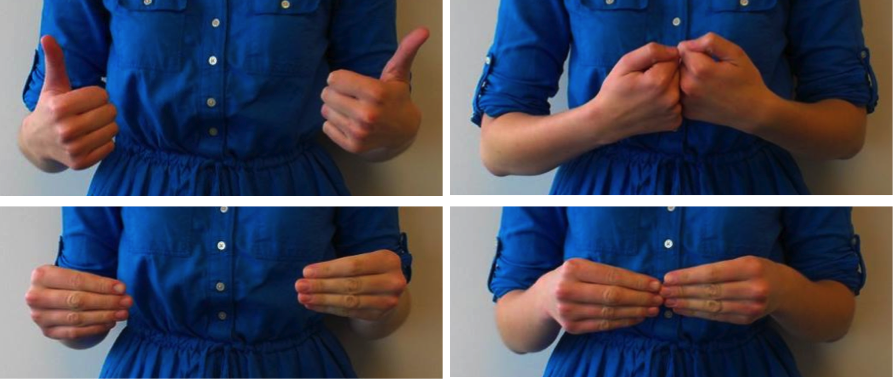
\includegraphics[scale=1]{MORESWEETHEART.png}
  \caption[Example of Signs with Similar Motion]
  { Example of Signs with Similar Motion.  \\ Top: SWEETHEART, Bottom: MORE  }
  \label{fig:MORE}
\end{figure}

The above examples represent only a small sampling of approaches that have been taken to solve the problem. Other techniques used for ASL recognition include Bayesian networks, [7] neural networks, [8] support vector machines [9] and several examples of Hidden Markov Models. [10][11] Some have also attempted to incorporate non-manual markers, small gestures of the face, eyebrows and shoulders meant to convey grammar and context, using face detection and computer vision techniques. [12]

\subsection{Scope}
This project encompasses the detection and tracking of a user's hand and finger gestures with the aim of developing an algorithm to be used in the automated detection of ASL as a teaching tool for learning ASL as a second language. To accommodate a group size of two members, and a time constraint of less than eight months, the project scope has been limited to the implementation of an existing hand- and finger-detection system and the development of a real-time gesture-recognition algorithm. Third-party solutions, such as existing hand- and finger-tracking or machine learning libraries, will be included as components wherever possible. 

Due to the constraints of this project, some or all of the following simplifying assumptions will be applied:
\begin{enumerate}
  \item The user interface will be minimal but will illustrate the basic structure of the tool, including demonstrating signs and testing the user. 
  \item The background of the user will be simplified or uniform, such as a blank wall. 
  \item Users may be required to wear artificial markers such as gloves or stickers.
  \item The project will focus on matching isolated, rather than continuous, signs. This will include classification of single words and short phrases but not whole sentences. 
\end{enumerate}

\newpage
\section{Design Objectives and Requirements}

\subsection{Objectives}
Our main goal is to demonstrate the technical feasibilty of an ASL teaching tool. From this perspective, our main objectives are to build a classification system that could reliably function as the backend to such a tool and provide an interface by which other developers could create applications. As a secondary objective, we would also construct a simple vocabulary game, to demonstrate the potential of the platform.

\begin{table}[h!]
\centering
\caption{Objectives}
\label{table:Objectives}
\vspace{1em}
\begin{tabular}{|c| p{14cm} |}
	\hline
	O.1 & Create a classification model that is accurate and robust \\ \hline
	O.2 & Create an API for using the classification model and an example application of the API in a teaching application \\ \hline
\end{tabular}
\end{table}

\subsection{Requirements}
The requirements outlined below in Table \ref{table:Requirements} are the result of literature review. They are tentative and are expected to undergo revision on the completion of interviews with potential users and stakeholders. The Regional Information Officer for the Canadian Hearing Society in Kitchener-Waterloo has contacted an ASL instructor from Conestoga College on our behalf.

\begin{table}[h!]
\centering
\caption{Requirements}
\label{table:Requirements}
\vspace{1em}
\begin{tabular}{|c| p{14cm} |}
	\hline
	R.1 & The video frame must encompass the body parts and surrounding area used when signing, i.e. the signer’s hands, head and shoulders. \\ \hline
	R.2 & The video frame not only must encompass the signer’s face, but must be sufficiently focused on the signer’s facial features in order for a viewer to make out the signer’s facial expressions.This is important not only because Non-Manual Markers form an important part of ASL grammatical structure [1], but also because not maintaining eye contact while communicating with ASL is viewed as rude and uninterested [2]. \\ \hline
	R.3 & The method used to capture the location and position of the signer’s hands must function for the speed at which a typical ASL user signs. \\ \hline
	R.4 & Hardware necessary to run the solution should be typical or inexpensive and easy to acquire. Either a user could be expected to already own the necessary hardware (example: commonplace laptop and webcam) or the required hardware is on the market and within the financial range of a middle-class person (example: Kinect or Leap Motion sensors). \\ \hline
	R.5 & Classification should occur in near real-time. Lag should not impede user engagement. \\ \hline
	R.6 & The solution should correctly identify signs with at least a 80\% success rate. \\ \hline
	R.7 & The solution should function in all common household lighting conditions without loss of speed or accuracy. \\ \hline
\end{tabular}
\end{table}

\subsection{Constraints}
The constraints on this project are described below in Table \ref{table:Constraints}. Constraints 3 and 4 necessitate allocating a large amount of time to research.

\begin{table}[h!]
\centering
\caption{Constraints}
\label{table:Constraints}
\vspace{1em}
\begin{tabular}{|c| p{14cm} |}
	\hline
	C.1 & Limited time; the project must be completed by March, 2014, while group members have additional obligations for courses and extracurriculars. \\ \hline
	C.2 & Small group size; two group members. \\ \hline
	C.3 & Limited previous experience of both group members with American Sign Language. \\  \hline
	C.4 & Limited previous experience of both group members with feature extraction methods, classification methods, and state-of-the art. \\ \hline
\end{tabular}
\end{table}

\newpage
\section{System Design}
The classification system follows the overall process shown in Figure \ref{fig:Process}, where the user input is the act of performing a sign in ASL. Starting with the raw data from our input device, video preprocessing is used to segment the image and reduce noise. Feature extraction methods are then used to extract relevant information- in this case, this could be the location, shape, or trajectory of the users hand. The information extracted will depend on what sign classification method is used to determine which sign the user has performed. This result is then displayed back to the user in some form.

\begin{figure}[h!]
  \centering
  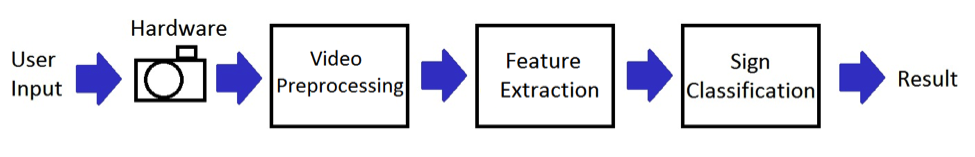
\includegraphics[scale=1]{Process.png}
  \caption{Breakdown of Sign Classification Process}
  \label{fig:Process}
\end{figure}

Within our scope, the four main design decisions that must be made are:
\begin{enumerate}
	\item The hardware used to collect raw data 
	\item The video preprocessing methods 
	\item Feature extraction methods 
	\item Sign classification methods. 
\end{enumerate}
Multiple methods may be implemented for each item. The following sections detail the current state of the system and the decision-making process up to this point.

\subsection{Hardware}
The visual input device chosen for this project must adhere to Requirement 4 (see Section 2), but also provide enough data to satisfy Requirement 6. 

The Microsoft Kinect is the hardware currently implemented in the prototype solution. The Kinect contains a camera that works either with a resolution of 1280x960 DPI and 
12 FPS, or 640x480 DPI and 30 FPS. It also includes an infrared emitter and depth sensor, enabling the device to get information on the depth of objects relative to the sensor. Though more expensive than a webcam, it is a commonly owned device. The XBOX Kinect can interface with a computer using a USB adapter.

The Kinect was chosen as an input device over other cameras and webcams due to the potential advantages given by its additional sensors. Currently our system only makes use of the Kinect camera, so it is possible for the code to be modified to accommodate a simple webcam. However, in the future we intend to make use of the Kinect’s depth sensors in order to increase classification accuracy and the number of signs that can be recognized.

In addition to the developer SDK, there is a cross-platform, open-source library for the Kinect called libfreenect. Libfreenect provides access to all of the Kinect’s sensors, and includes Fakenect, a utility that allows the user to record Kinect data to be used later (“faking” a Kinect data stream). Using Fakenect, several trials of each sign can be recorded to be used later in creating a classification model. While libfreenect does not provide access to all the APIs included in the developer SDK, such as skeletal tracking, we have found it to be preferable for rapid prototyping as it allows us to incorporate other open-source libraries, such as OpenCV, and to make use of the Fakenect utility for recording classifier training data.

\subsection{Colour Recognition and Preprocessing}
The current solution uses a coloured glove and a series of filters to get the position of the hand and fingers. 

\subsubsection{Use of Markers}
The hand-tracking libraries in Table \ref{table:libraries} were investigated. These libraries are intended to identify a user’s bare hand. None of the libraries were found to be usable for the purposes of this project, and instead a glove with artificial markers will be implemented.

\begin{table}[h!]
\centering
\caption{Hand-Tracking LIbraries}
\label{table:libraries}
\vspace{1em}
\begin{tabular}{|p{5cm}| p{11cm} |}
\hline
\textbf{Name/Company} & \textbf{Capabilities} \\ \hline
3D Hand Tracking by The Foundation for Research and Technology-Hellas (FORTH) [3] &
Creates a model of the hand that is capable of tracking individual fingers without losing them when out of site.
Advertises no calibration required \\ \hline
TuioKinect hand tracker for Kinect [4] &
Can recognize large hand gestures but does not have individual finger recognition. \\ \hline
Hand Kinetics [5]  &
Hand and segment model created with classifiers appears to capture fingers very well. Not yet commercially available. \\ \hline
\end{tabular}
\end{table}


The Hand Kinetics application is not yet commercially available. The TuioKinect hand tracker does not support finger recognition and therefore not capable of collecting sufficient data to create an accurate classifier. The library by FORTH could not reliably track a hand as demonstrated in Figure \ref{fig:FORTH}. 

\begin{figure}[h]
  \centering
  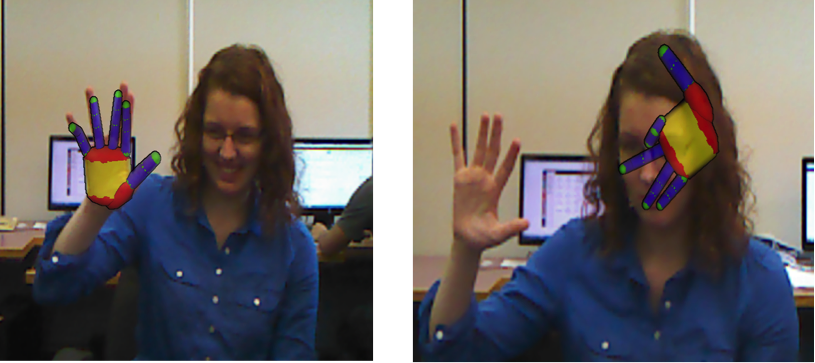
\includegraphics[scale=1]{FORTH.png}
  \caption{Example of an Existing Hand-Tracking LIbrary}
  \label{fig:FORTH}
\end{figure}

The difficulty in tracking a bare hand is due to several factors. First, skin colour differs widely between people. When a person’s face is also in the frame, an algorithm may be unable to differentiate between the facial skin and the skin of the hand. It is also difficult to identify fingers and fingertips from the rest of the hand, specifically when a user’s fingers overlap the palm, such as in the ASL sign for the letter ‘A’.

The use of a glove solves the problem of differentiating skin colours, and allows the application of artificial markers to identify specific regions of the hand such as the fingertips or palm. In the realm of a teaching application, requiring a user to wear a glove is reasonable provided the glove does not inhibit the user’s motion and does not impose a significant increase in cost. 

\subsubsection{Glove and Marker Design}
A simple knit glove was selected for the glove base. This type of glove is inexpensive and available in many colours. Our intent was to add additional coloured markers to the glove to serve as landmarks for video preprocessing. The initial design of the gloves is described in Figure \ref{fig:glove}.

\begin{figure}[h]
  \centering
  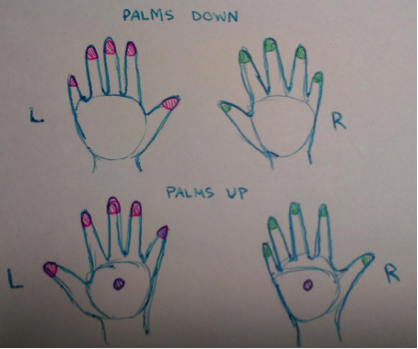
\includegraphics[scale=1]{GloveDesign.png}
  \caption{Initial Glove Designs}
  \label{fig:glove}
\end{figure}

Initially, markers (pink and green in the above figure) were to be made using fabric paint. This was attempted on gloves, but the paint was found to be uneven, lumpy and far too reflective. The finger tips were difficult to identify using filters because the colour was too variable, depending greatly on the angle with respect to the light sources. Instead, felt finger caps were sewn. 

In order to determine the best colours to use for the gloves and fingertip markers, colour separability was examined in YCbCr, a colour spaces that separates illumination from chroma. This is important for robustness across illumination (Requirement 7). 

\begin{figure}[h]
  \centering
  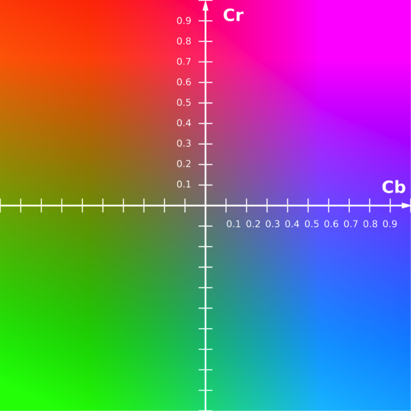
\includegraphics[scale=1]{YUV.png}
  \caption{CbCr Plane at Y = 0.5}
  \label{fig:YUV}
\end{figure}

According to the graph, the most separable colours should be red, green, magenta and blue. Colours of this purity are not available as materials, and so testing was done to identify the most separable colours independent of lighting. Seven different colours were tested (six as fingertip caps, and one as the glove colour).

\begin{figure}[h]
  \centering
  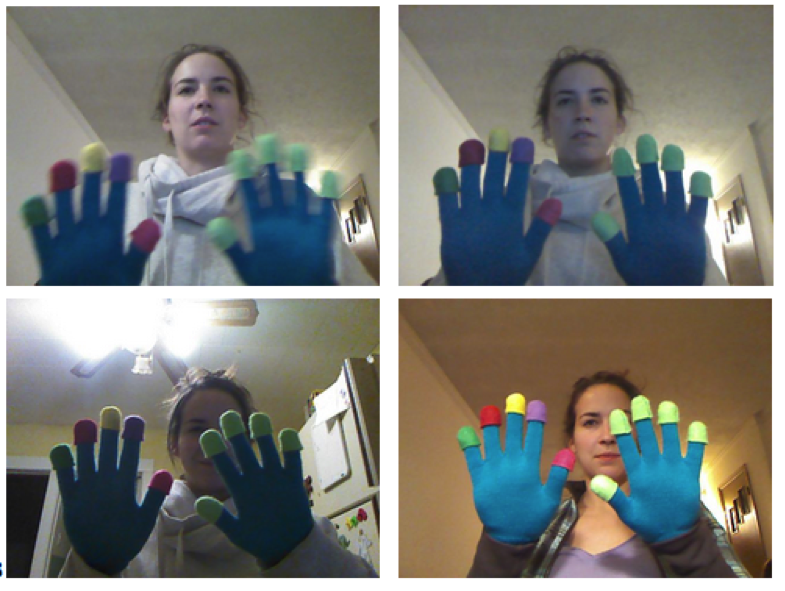
\includegraphics[scale=1]{LightTest.png}
  \caption{Illumination Tests}
  \label{fig:light}
\end{figure}

Images in four different illumination settings (ambient, dark ambient, back-lit and front-lit) were used to calculate test means for each colour based on 900 sample pixels. (Figure \ref{light}) A second test image for each illumination was then used to classify colours based on euclidian distance to the test means. The resulting confusion matrices can be found in Appendix A.

Figure \ref{fig:YUVTest} shows a visualization of the location of 900 samples in one test image in the CbCr space. 

\begin{figure}[h]
  \centering
  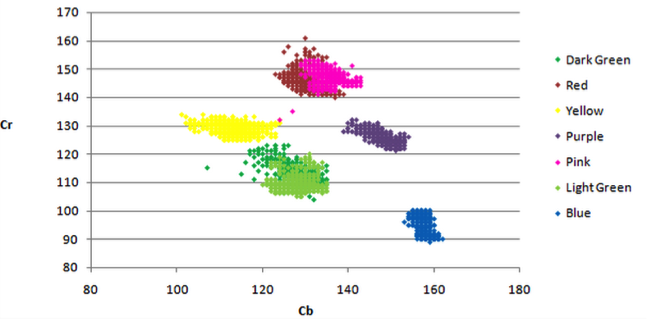
\includegraphics[scale=1]{YUVTest.png}
  \caption{Colour Samples in the CbCr Plane}
  \label{fig:YUVTest}
\end{figure}

The following conclusions were drawn based on the confusion matrices analysis: 
\begin{enumerate}
	\item Dark Green and Light Green are often misclassified as one another 
	\item Red and Pink are often misclassified as one another
	\item Yellow is occasionally misclassified as Light Green
	\item Purple is occasionally misclassified as Blue
	\item Blue is the most reliably separable colour of the seven colours tested
\end{enumerate}

Colours were also tested qualitatively for salience against the background (including the user’s face). Results showed that colours can be satisfactorily identified from the background with this tolerance using filters, provided the user is not wearing a shirt within that tolerance of the colour in question. The results also demonstrated that colours that can be misclassified should not be implemented together. Figure \ref{fig:salience} shows a binary filter identifying Light Green (but also picks up Dark Green). 

\begin{figure}[h]
  \centering
  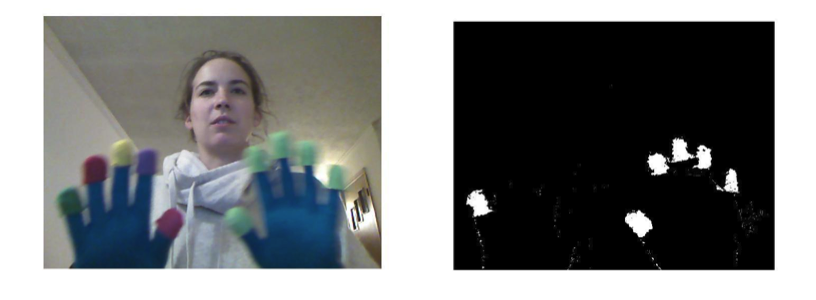
\includegraphics[scale=1]{BinaryTest.png}
  \caption{Colour Detection}
  \label{fig:salience}
\end{figure}

To identify finger markers, a binary filter is applied, followed by size and eccentricity filters to reduce noise, and then a hole-filling algorithm.

Based on our analysis, the colours used in the gloves should be: \\
\hspace*{1cm} Blue gloves \\
\hspace*{1cm} Light Green fingertips on the right hand (current prototype) \\
\hspace*{1cm} Red fingertips on the left hand (future)


Calibration is achieved by manually selecting green section in a frame, and then an algorithm stores the acquired information in a CSV document, to be used in conjunction with the classifier.

\subsubsection{Next Steps}
The following are goals to be implemented by March 2014:
\begin{enumerate}
	\item The second glove will be created.
	\item Colour tolerance may be investigated in order to minimize the sensitivity to lighting changes.
	\item Colour detection will be made more robust, possibly through techniques such as segmentation
	\item If still required, calibration will be automated. 
	\item If required by the final feature extraction and classification methods, additional markers may be added to the gloves.
\end{enumerate}

\subsection{Feature Extraction and Classification}
As can be seen in the research, there is no shortage of well-studied labelled classification methods that can be used in gesture recognition applications. However, selecting the best classifier for a problem is a non-trivial exercise. In addition, all of these methods require that our processed video data first be distilled into a series of meaningful, quantitative values known as the feature set. The selection of appropriate features is another non-trivial endeavour as the use of meaningful metrics has a drastic effect on classifier skill.

In our initial prototype, we chose to classify signs based solely on individual frames. This allows us to classify ‘static’ signs such as the letters of the ASL alphabet but it is not sufficient to classify motion-based signs, including most vocabulary words. We hope to be able to recognize motion-based signs in future prototypes. 

Building a classifier also required us to construct a library of labelled data. To construct the library, each of the developers recorded a series of short fakenect data samples of themselves signing single letters while wearing the glove in various lighting conditions. Due to the amount of time required to record this data, we chose to limit ourselves to recognizing only a subset of the alphabet. Our current library includes the letters: A, B, C, E, F, G, H, M, and N. This recorded library if used by the classifier to “learn” the feature vectors associated with these labels, a process known as training.  

\subsubsection{Model Validation}
There are several metrics by which we can determine the predictive skill of a classifier. The simplest is accuracy, which here refers to the percentage of correctly classified signs within some sample set. For each class, we can also measure the precision and recall, defined as:
\begin{gather*}
\text{precision} = \frac {\text{true positives}} {\text{true positives} + \text{false positives}} 
\quad \quad
\text{recall} = \frac {\text{true positives}} {\text{true positives} + \text{false negatives}}
\end{gather*}
These two metrics give precision as the ratio of samples predicted as class A that actually belong to class A, and recall as the ratio of samples belonging to class A that were predicted as being class A, respectively. Finally, for a multiclass classifier, we can output a confusion matrix, which gives a detailed breakdown of all predictions against their actual labels. 

Furthermore, there are two ways of producing a sample set for calculating these metrics. Given a library of labelled samples with which to train a classifier, we can split it into a training set and a test set; we use the training set to build the classifier and then try to predict the samples in the test set, to determine how well the classifier generalizes to new information. Alternatively, we can split the samples into a number of folds; we build a classifier using all but one fold, then predict the single remaining fold with the resulting classifier. This technique is known as cross-validation.  

In our experiments, test accuracy is used as the main indicator of predictive skill; however, precision, recall and confusion matrices are useful for diagnosing the shortcomings of specific classifiers. These metrics can be used to motivate decision-making about the selected features and classifier, as detailed in the following sections. 

\subsubsection{Selection of Classifier}
For our initial prototype, we chose to use a support vector machine (SVM) classifier. This was chosen mainly because the developers are already familiar with training support vectors machines, they are widely used in industry including in our literature review, and the intuition behind them is simple. 

Every labelled sample in our training library has a single feature vector of length n associated with it; these can be viewed as points within an n-dimensional feature space. During training, the support vector machine constructs a series of hyperplanes to separate points belonging to different classes; this plane serves as the class boundary when predicting future samples. The goal of the SVM is to maximize the margin between the boundary and the nearest points on either side. 

\begin{figure}[h!]
  \centering
  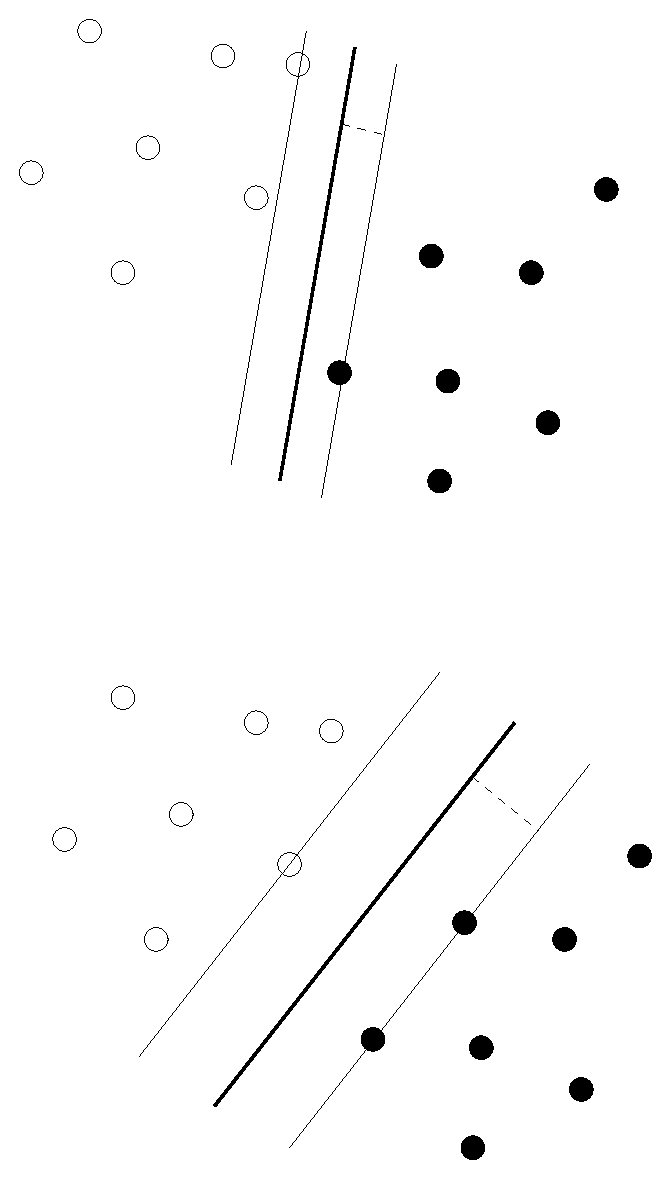
\includegraphics[scale=1]{classifier}
  \caption[Illustration of an SVM Decision Boundary]
   {Illustration of an SVM Decision Boundary. \\ Above: a non-optimal boundary, Below: an optimal boundary with wider margins}
  \label{fig:Classifier}
\end{figure}

Since these data are not always linearly separable, a few modifications exist to make the classifier more flexible: the C parameter and kernel functions. 

The C parameter controls the cost associated with misclassifying a sample in the training set. As C increases, higher priority is placed on correctly classifying all samples in the training set; as C decreases, higher priority is placed on maximizing the margins.

Using a kernel function maps the training set into a higher dimensional feature space. This allows the SVM to create boundaries that are more complex in the original feature space. One of the most common kernel functions is the radial basis function; the effect of this kernel is to create “force fields” around individual samples which influence the path of the decision boundary. When using the radial basis function, there is an additional parameter, \(\gamma\), which controls the smoothness of the boundary.

\begin{figure}[h]
  \centering
  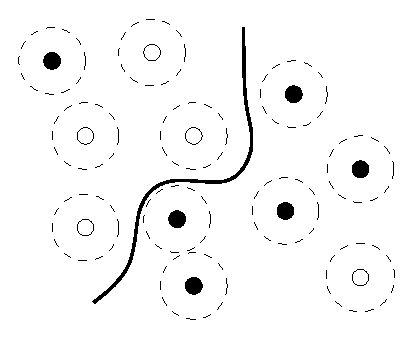
\includegraphics[scale=1]{rbf}
  \caption{Example RBF Decision Boundary}
  \label{fig:RBF}
\end{figure}

When building a classifier, it is necessary to choose a C parameter, a kernel function, and, if necessary, a \(\gamma\) that maximizes the predictive skill of the classifier. We chose to use a grid-search method to automate this process. In grid search, a series of possible values are selected for each parameter. The classifier is trained using every combination of these parameters and the classifier selected is the one with the best cross-validated accuracy. 

The parameter search space is given in Table \ref{table:gridsearch}. For kernel functions, we used only the linear and radial basis function kernels. Both C and gamma increase by powers of ten, searching a wide range but using only a handful of values. Grid search is run every time a new classifier is constructed. Results for individual trials are given in Appendix B.

\begin{table}
\centering
\caption{Grid Search Parameter Values}
\label{table:gridsearch}
\begin{tabular}{ |l|l| }
\hline
\textbf{Parameter} & \textbf{Values} \\ \hline
\( C \) &  1, 10, 100, 1000, 10000 \\ \hline
kernal & \textit{linear}, \textit{rbf} \\ \hline
\( \gamma \) & 0.01, 0.001, 0.0001, 0.00001 \\ 
\hline
\end{tabular}
\end{table}

\subsubsection{Selection of Features}
After processing the input from the Kinect, we are left with a binary image of the glove markers. The next task is to develop some meaningful set of features describing the binary image, for use in classification. Possible features include the size and shape of the binary blobs or the positions and relatives distances of blob centroids as well as more complex image processing features such as eigenvectors, Haar-like features, and Fourier descriptors. We chose to begin by testing the predictive skill of some simple shape descriptors.

First, we connect all the marker blobs into a single shape by taking the convex hull. The convex hull is the smallest shape that contains all of the marker blobs but also has no convexity defects along its perimeter. The result is a single shape that describes, hopefully, the relative positions of all the fingers visible in the frame. 

\begin{figure}[h]
  \centering
  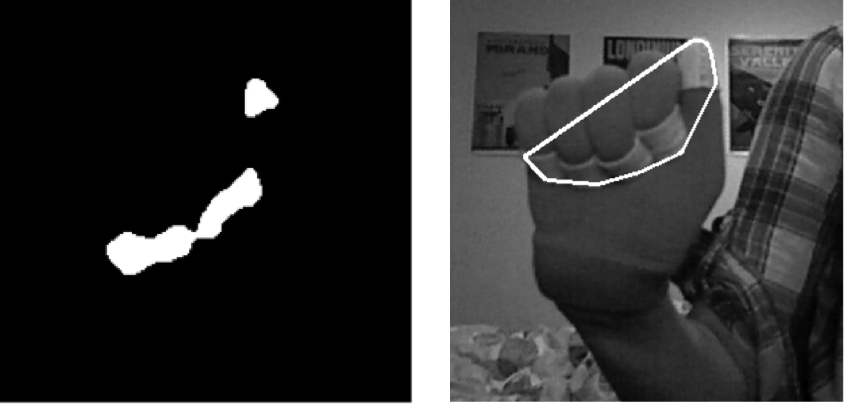
\includegraphics[scale=1]{Hull.png}
  \caption{Convex Hull from Binary Image}
  \label{fig:hull}
\end{figure}

We can convert this shape into a feature vector using shape descriptors. In our experiments, we used three different types of image moments: central moments, Hu moments and Zernike moments.

The central image moments are perhaps the simplest image descriptors; they describe the distribution of a shape about its x and y axes. Each raw moment, \(M_{pq}\), is defined as follows:

\dothis{Equation}

We use the central normalized moments, \({n\mu}_{pq}\), which have been normalized and repositioned, making them both shift- and scale- invariant. This is a necessary feature of all our image descriptors; recognition of the sign should be independent of the hand’s position in the frame, or distance from the Kinect.  When classifying signs we use the first seven central moments. ( \(p+q \leq 3\) )

Hu moments are another set of image moments, notable for being rotation-invariant in addition to shift- and scale-invariant. The first seven Hu moments are calculated from the first seven normalized central moments.

The Zernike moments are constructed from the Zernike polynomials and designed to be completely orthogonal. They have been shown to outperform other descriptors in terms of information redundancy and image representation. \dothis{(Ref)} The first seven moments are constructed as follows:

\dothis{Equations}

Upon testing all three descriptors, we immediately found that the Zernike moments were too complex to be calculated in a reasonable amount of time. Training took hours but, more importantly, the moments could not be calculated fast enough to perform sign recognition in real time. This trial was put aside pending research into fast calculations. Of the two remaining shape descriptors, the central moments consistently perform better than the Hu moments, as shown in Appendix B. This is unsurprising as signs have a definitive orientation and there is typically very little rotation of the hand while signing the alphabet. Using a rotation-invariant feature set removes key information about the orientation of the fingers. 

\subsubsection{Next Steps}
There are several improvements that we wish to make in future iterations of our prototype, including the use of addition feature sets in our static classifier. The most important of these is the inclusion of temporal features, which would allow us to classify vocabulary words and motion-based signs. These could include tracking hand trajectories, as in the recent, or using frame-to-frame changes in hand posture. The inclusion of these features will likely also warrant the use of more elaborate classifiers; Hidden Markov Models, for example are widely used. Additional research will be required to select the appropriate features and classifiers. By March we hope to have a new classifier working, using an expanded feature set, which would be capable of identifying a small library of vocabulary words.

\subsection{User Interface Mockup}
The teaching tool system detects the satisfactory completion of a sign. This system is intended to be implemented in a number of ways: an ASL-to-English dictionary, or a vocabulary game.

By March 2014, a simple call-and-response vocabulary game will be created to exemplify a possible use of the system. Figures \ref{fig:ui1} and \ref{fig:ui2} demonstrate how the user will interact with the game.

\begin{figure}[h]
  \centering
  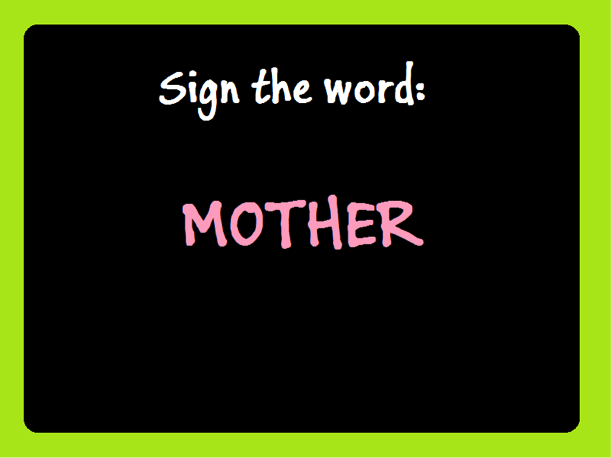
\includegraphics[scale=1]{Mother.png}
  \caption{UI Mockup: Prompting }
  \label{fig:ui1}
\end{figure}

\begin{figure}[h]
  \centering
  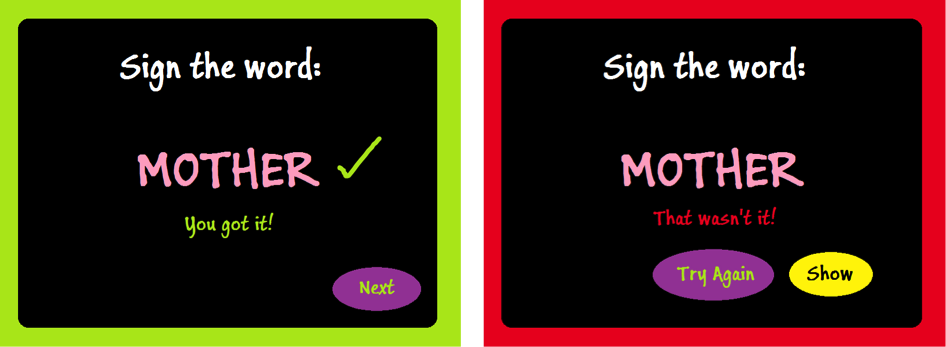
\includegraphics[scale=1]{Mother2.png}
  \caption{UI Mockup: Feedback}
  \label{fig:ui2}
\end{figure}

If the system recognizes a match between the sign the user performed and the sign being tested, then the user is given positive feedback and is allowed to proceed to the next vocabulary sign. If the system does not recognize a match, the user signed the wrong word. The user is given the option to try again, or be shown a short instructional video on how to make the sign. 

\newpage
\section{Project Progress and Schedule}
\subsection{Timeline}
The Gantt chart in Figure \ref{fig:gantt} has been updated from the one submitted with the Design Plan to include additional milestones for the Winter 2014 term. Otherwise, very little has been edited because the project is on track with the projected timeline. The main difference between the original project plan and the current progress is that each major section has become an iterative process. For instance, feature selection and extraction is highly tied to the performance of the classifier, and will therefore selection of features will continue at the same time as classifier experimentation. Feature selection may also affect the glove design, should additional markers end up being desirable. 

\begin{figure}[h!]
  \centering
  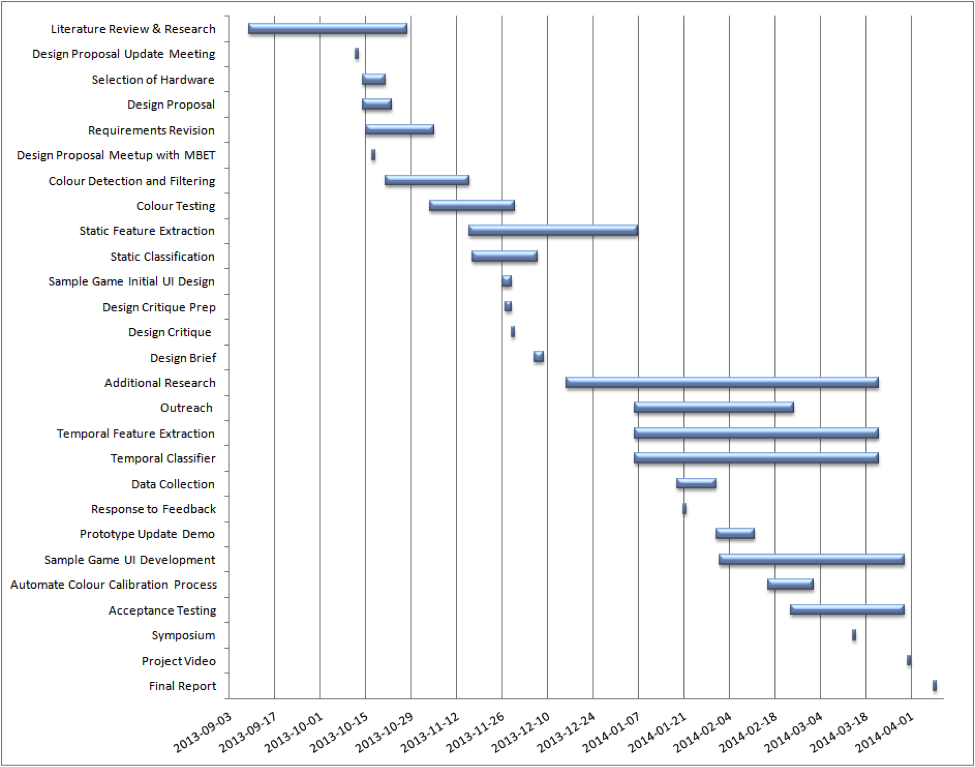
\includegraphics[scale=1]{Gantt.png}
  \caption{Updated Gantt Chart}
  \label{fig:gantt}
\end{figure}

Individual contributions and future responsibilities of each group member can be found in Section \ref{subsec:member}.

\subsection{Progress}
The milestones listed below have been completed. Video preprocessing methods include the glove design as well as colour detection, filtering and testing. The approval of this application is necessary to commence gathering video data from potential users other than the project group members. The same application encompasses user testing to assess the usability and educational value of the final prototype. The initial review has already been received and the necessary edited documents have been re-submitted. Approval is anticipated for January.

\begin{enumerate}
  \item Revised design requirements
  \item Selection of hardware
  \item Video preprocessing methods selected
  \item Feature extraction research and first prototype implementation
  \item Simple classifier implementation
  \item Manual calibration system
  \item User interface mockup
  \item University of Waterloo Ethics Approval application submission
\end{enumerate}

The following milestones will be completed in the Winter 2014 term:
\begin{enumerate}
  \item Acquisition of user data
  \item Selecting a set of signs to be used in the final prototype
  \item Experimentation with additional features
  \item Classification of dynamic signs
  \item Experimentation with other classification methods
  \item Automated calibration 
  \item Outreach component
  \item Project video
  \item Final prototype
  \item Acceptance testing
\end{enumerate}

\newpage
\section{Project Management}
\subsection{Member Contributions}
\label{subsec:member}
This term Sara was responsible for colour analysis and testing, glove design, user interface mockups, meeting minutes, communication with supervisors, and the research ethics approval application. 

Jennifer was responsible for leading the literature review and the development and testing of the initial feature extraction and classification techniques. 

Jennifer and Sara collaborated on the preparation of the Dragon’s Den demo, and much of the decision making was shared.

In the following term, Sara will continue to take meeting minutes and arrange communication with supervisors. She will also take responsibility for user data collection and acceptance testing. 

Jennifer will head feature extraction and classification research and experimentation. 

Jennifer and Sara will share responsibility of developing the final prototype, including the creation of a simple user interface. Decision making will continue to be a group activity. 

\subsection{Document Management}
Meeting minutes, brainstorming and progress are stored in a shared Google Documents folder. This folder serves as a digital notebook for both group members. A repository on GitHub is used for project code and version control. Because the Kinect video data used to create a classification model is so large, a subscription dropbox folder stores this data as a backup to the data stored on an external hard drive. 

\subsection{Group and Supervisor Meetings}
The group met with the supervisors once a week, for 15-30 minutes. Group members met officially 1-2 times a week, but updates and discussion occurred frequently and organically due to living in the same residence. This system was effective and will continue in the following term. 

\subsection{Financial Budget}
Hardware (personal computers and Kinect camera) were possessed by group members prior to the project and are therefore not included in the budget. Likewise, software libraries are all open source and have no financial cost. The financial budget is allocated towards glove materials and a monthly dropbox fee, used for sharing the large training library between group members. 

\begin{table}[h!]
\centering
\caption{Budget}
\label{table:Budget}
\vspace{1em}
\begin{tabular}{l r}

\textbf{Item}  & \textbf{Cost} \\ \hline
3 pairs of gloves, fabric paint, 7 sheets of felt,craft glue & \$30.00 \\
Dropbox subscription for additional space, \$10/month for 6 months & \$60.00 \\ \hline
Total & \$90.00 \\
\end{tabular}
\end{table}

\subsection{Facilities}
No special facilities are required for this project.

\subsection{Resources}
A number of external information resources are available. One of the directors at the Vision and Image Processing Lab at the University of Waterloo is a supervisor for this project, and the remaining supervisor is a graduate student in the same lab. They both offer guidance and support for the technical aspects of the project. In addition, we have been allowed to borrow a Kinect from the Image Processing Lab.

A contact at the Canadian Hearing Society is willing to answer questions by phone and by email.

\newpage
\section{Conclusion}

\newpage
\tocsection{Appendix A - \dothis{Thing}}

\newpage
\tocsection{Appendix B - \dothis{Thing}}




\end{document}